\documentclass{article}
\usepackage{graphicx}
\usepackage{float}
\usepackage{hyperref}
\graphicspath{ {images/} }

\title{
    Software Requirements Specification\\
    \begin{large}
        \textit{Golf Course Mapper}
    \end{large}
}
\date{
    \begin{small}
        \today
    \end{small}
}
\author{
    Team Recursive Recursion
}

\begin{document}
    \pagenumbering{gobble}
    \maketitle
    \newpage

    \tableofcontents
    \newpage

    \pagenumbering{arabic}

    %===========================================================================
    
    \section{Overview}

    \subsection{Purpose}

    This Software Requirements Specification (henceforth SRS) is intended to be
    a guide on the path of developing the Golf Course Mapper system. It will
    aid the developers by providing a layout of the project requirements.

    \subsection{Scope}

    Golf players require an application that allows them to view golf courses
    during play. Although there are existing platforms that aim to achieve this
    goal, many of them are simply mappers and do not allow the player to view
    their location on the map.
    
    Furthermore, the proprietary and commercial nature of existing products
    make them difficult to be used widely and therefore contain only a handful
    of mapped courses. The Golf Course Mapper will attempt to achieve these
    goals by providing a rich set of features for both the course managers and
    players through an open source platform.

    The Golf Course Mapper will allow golf course managers to draw the shape of
    their courses using a web application. The owners will map out the details
    of the golf course. This includes mapping the layout of the fairway, green,
    sand and water hazards and details such as the position of the hole and the
    teeing grounds. Additionally, owners will be allowed to view their courses
    and see the locations of active players currently using either the Android
    or iOS mobile applications.

    Players currently on the course will be able to use the provided mobile
    applications to view the map of the course and their current location on
    the course. This has the benefit of allowing players to plan their shots
    more strategically. The app will show the distances between the player and
    various points of interest (such as the hole), further aiding the player
    during play.

    The Golf Course Mapper is not a coaching tool and does not provide a
    channel of communication between the mapper and the player, nor does it
    provide any communication between players. The web application is not to be
    used by coaches, but solely by managers that wish to map out the details of
    their courses and view its current state. The Golf Course Mapper is also
    not a social media platform for golfers and will not allow communication
    among any involved parties.

    \subsection{Definitions, Acronyms \& Abbreviations}
    \begin{itemize}
        \item
            System: Henceforth used to refer to the Golf Course Mapper system
            as a whole.
        \item
            Manager: The manager or owner of a golf course, henceforth used to
            refer to the user of the website.
        \item
            Player: A golf player, henceforth used to refer to the users of the
            mobile applications.
        \item
            Website: The web application that is used by golf course managers
            to draw the layout of their golf courses.
        \item
            Android App: A native Android mobile app that golf players can use to
            view the golf course.
        \item
            iOS App: A native iOS mobile app that golf players can use to view
            the golf course.
        \item
            Location: A position on the map, modelled using latitude and longitude
            coordinates.
        \item
            Point: A point of interest, such as the hole or tee location.
            Points are represented as a single location on the golf course.
        \item
            Area: Specific areas on the golf course, such as the green or the
            fairway. Areas consist of a cyclically ordered set of locations,
            forming a polygon.
        \item
            DBMS: Database Management System.
        \item
            API: Application Programming Interface.
        \item
            Back End: The server side that consists of both the DBMS and the
            API.
    \end{itemize}

    \subsection{Domain Model}

    Refer to figure \ref{fig:domainmodel}, which represents the domain model of
    the system. At the core of the domain model is the \textit{Course} which
    represents a single area where \textit{Players} can go to play the game of
    golf. Each Player is associated with a single Course on which the Player is
    currently playing. Each Course has an assigned \textit{Manager} that is
    solely responsible for mapping and managing the information of the Course.
    Note that a Manager can be assigned to more than one Course.

    Each Course has one or more \textit{Holes} associated with it. A Hole
    represents a single playable map with different map \textit{Elements},
    containing information. The Elements can be of two different types:
    \textit{Point} Elements and \textit{Area} Elements. A Point Element
    represents single-point information of a Hole such as the teeing grounds,
    location of the hole and other points of interest. Area Elements represent
    area information of a Hole, such as the area of the rough, fairway, green
    and water and sand hazards. Areas are represented as polygons.

    A Course may also optionally have Elements that are not associated with a
    specific Hole. This allows the specification of Elements such as points of
    interest or hazardous areas such as bodies of water that may be important
    to or span more than one Hole. It therefore does not make sense to
    associate these Elements with a specific Hole, but rather with the Course
    as a whole.
    
    \begin{figure}[H]
    	\centering
    	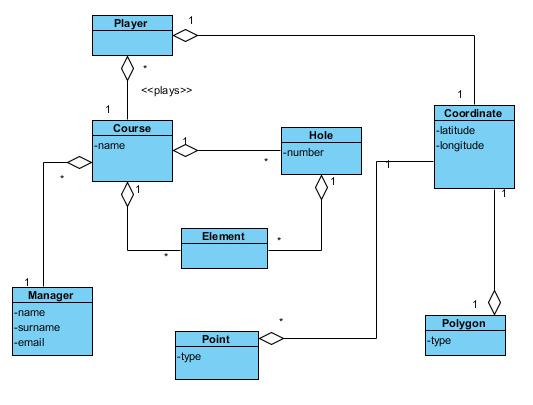
\includegraphics[scale=0.5]{DomainModel}
        \caption{Domain model of the system.}
        \label{fig:domainmodel}
    \end{figure}

    \newpage

    %===========================================================================

    \section{Functional Requirements} 

    \subsection{Users}

    The system contains two different users, listed below. Further details
    about functions that each user will perform are stipulated in Section
    \ref{sec:requirements}.

    \begin{itemize}
        \item \textbf{Manager:} These users are golf course managers or owners
            that use the web application. They primarily create or edit golf
            courses and view the positions of active players on the map. These
            users must be registered on the system and must be authenticated
            before being able to modify or create courses.
        \item \textbf{Player:} These users are golf players that use the mobile
            applications, primarily to view the course and receive contextual
            information. These users are anonymous and do not require any
            authentication to access the application.
    \end{itemize}

    \subsection{Subsystems}

    The system is composed of four subsystems, listed below. Further details
    about functions that each subsystem will perform are stipulated in Section
    \ref{sec:requirements}. The component diagram in figure \ref{fig:component}
    illustrates the subsystems and their relationships.

    \begin{itemize}
        \item \textbf{Android App:} This subsystem comprises of a native
            Android mobile application that is used to view mapped courses and
            other contextual information. The Google Maps API will be used for
            displaying the map received through the Zoning API, described
            below.
        \item \textbf{iOS App:} This subsystem comprises of a native iOS mobile
            application that is used to view mapped courses and other
            contextual information. The Google Maps API will be used for
            displaying the map received through the Zoning API, described
            below.
        \item \textbf{Web Application:} This subsystem comprises of in
            interactive web application for creating, mapping and editing
            courses, as well as viewing the location of currently active
            players. The Google Maps API will be used for drawing the map
            elements which are loaded and saved using the Zoning API, described
            below.
        \item \textbf{Zoning API:} This subsystem covers the backend of the
            system. This subsystem further contains the following two
            subsystems:
            \subitem \textbf{DBMS:} A PostgreSQL installation with the PostGIS
            extension, used to persist any mapping elements and other related
            information.
            \subitem \textbf{API:} A REST API using the Microsoft .NET Core
            Entity Framework, which will grant simple and secure access to the
            information stored in the DBMS.
    \end{itemize}

    \begin{figure}[H]
        \centering
        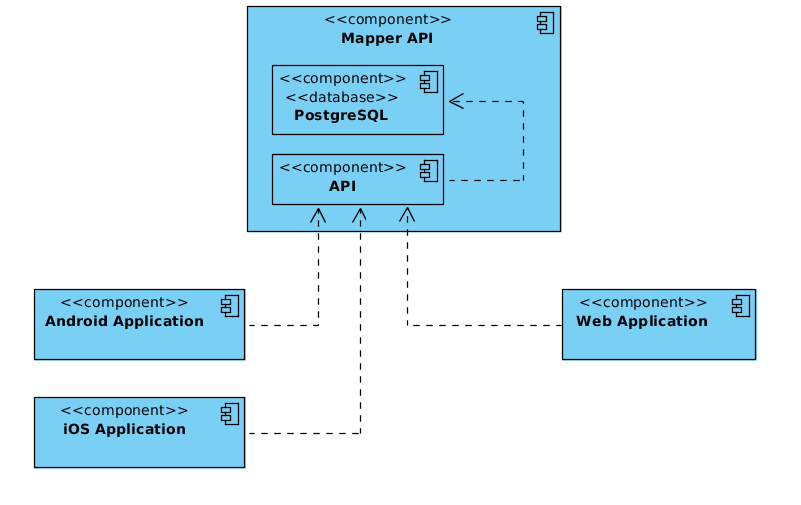
\includegraphics[scale=0.45]{ComponentDiagram}
        \caption{Component diagram illustrating subsystems.}
        \label{fig:component}
    \end{figure}

    \subsection{Specific Requirements}
    \label{sec:requirements}

    The following functional requirements describes the functionality that the
    system will provide. It is drawn from user stories that are also
    illustrated by the use case diagram in figure \ref{fig:usecase}.

    \begin{itemize}
        \item
            \textbf{R1} The manager will register to the website.
        \item
            \textbf{R2} The registered manager will log into the Website.
        \item
            \textbf{R3} The manager will manage courses.
            \subitem \textbf{R3.1} The manager will create new courses, given a
            name and a description.
            \subitem \textbf{R3.2} The manager will remove existing courses.
            \subitem \textbf{R3.3} The manager will select an existing course
            to edit.
            \subitem \textbf{R3.4} The manager will change the name and
            description of an existing course.
        \item
            \textbf{R4} The manager will control the holes on the course.
            \subitem \textbf{R4.1} The manager will add new holes to the
            course, given a name and the par of the hole.
            \subitem \textbf{R4.2} The manager will remove existing holes from
            the course.
            \subitem \textbf{R4.3} The manager will select an existing hole to
            edit.
            \subitem \textbf{R4.4} The manager will change the name and
            description of an existing hole.
        \item
            \textbf{R5} The manager will add areas to the active hole/course.
            \subitem \textbf{R5.1} The manager will choose to add a new area.
            \subitem \textbf{R5.2} The manager will draw a polygon on the map.
            \subitem \textbf{R5.3} The manager will select the type of the
            area.
            \subitem \textbf{R5.4} The manager will have the option to abandon
            the creation of the area.
        \item
            \textbf{R6} The manager will add points to the active hole/course.
            \subitem \textbf{R6.1} The manager will choose to add a new point.
            \subitem \textbf{R6.2} The manager will place a point on the map.
            \subitem \textbf{R6.3} The manager will select the type of the
            point and optionally enter additional info.
            \subitem \textbf{R6.4} The manager will have the option to abandon
            the creation of the point.
        \item
            \textbf{R7} The manager will edit existing elements (areas and
            points) on the active hole/course.
            \subitem \textbf{R7.1} The manager will edit a selected element by
            dragging the component(s) of the element.
            \subitem \textbf{R7.2} The manager will remove a selected element.
        \item
            \textbf{R8} The manager will enable the location view, which will
            display the locations of all current players (using the mobile
            apps) on the course.
        \item
            \textbf{R9} The player will view a course on the mobile app.
            \subitem \textbf{R9.1} The player will see a list of courses
            ordered by ascending distance from the player.
            \subitem \textbf{R9.2} The player will search for the name of a
            specific course.
            \subitem \textbf{R9.3} The player will choose a course to view on
            the map.
            \subitem \textbf{R9.4} The player will choose a specific hole to
            view on the selected course.
        \item
            \textbf{R10} The player will see his current position displayed on
            the map.
        \item
            \textbf{R11} The player will se contextual information.
            \subitem \textbf{R11.1} The player will see the distance between their
            current location and the current hole's flag.
            \subitem \textbf{R11.2} The player will see the name of the golf club
            that is recommended for the distance to the current hole's flag.
            \subitem \textbf{R11.3} The player will see the distance between
            their current location and any point of interest on the course by
            selecting the point.
    \end{itemize}
    
    % TODO activity diagram

    \begin{figure}[H]
        \centering
        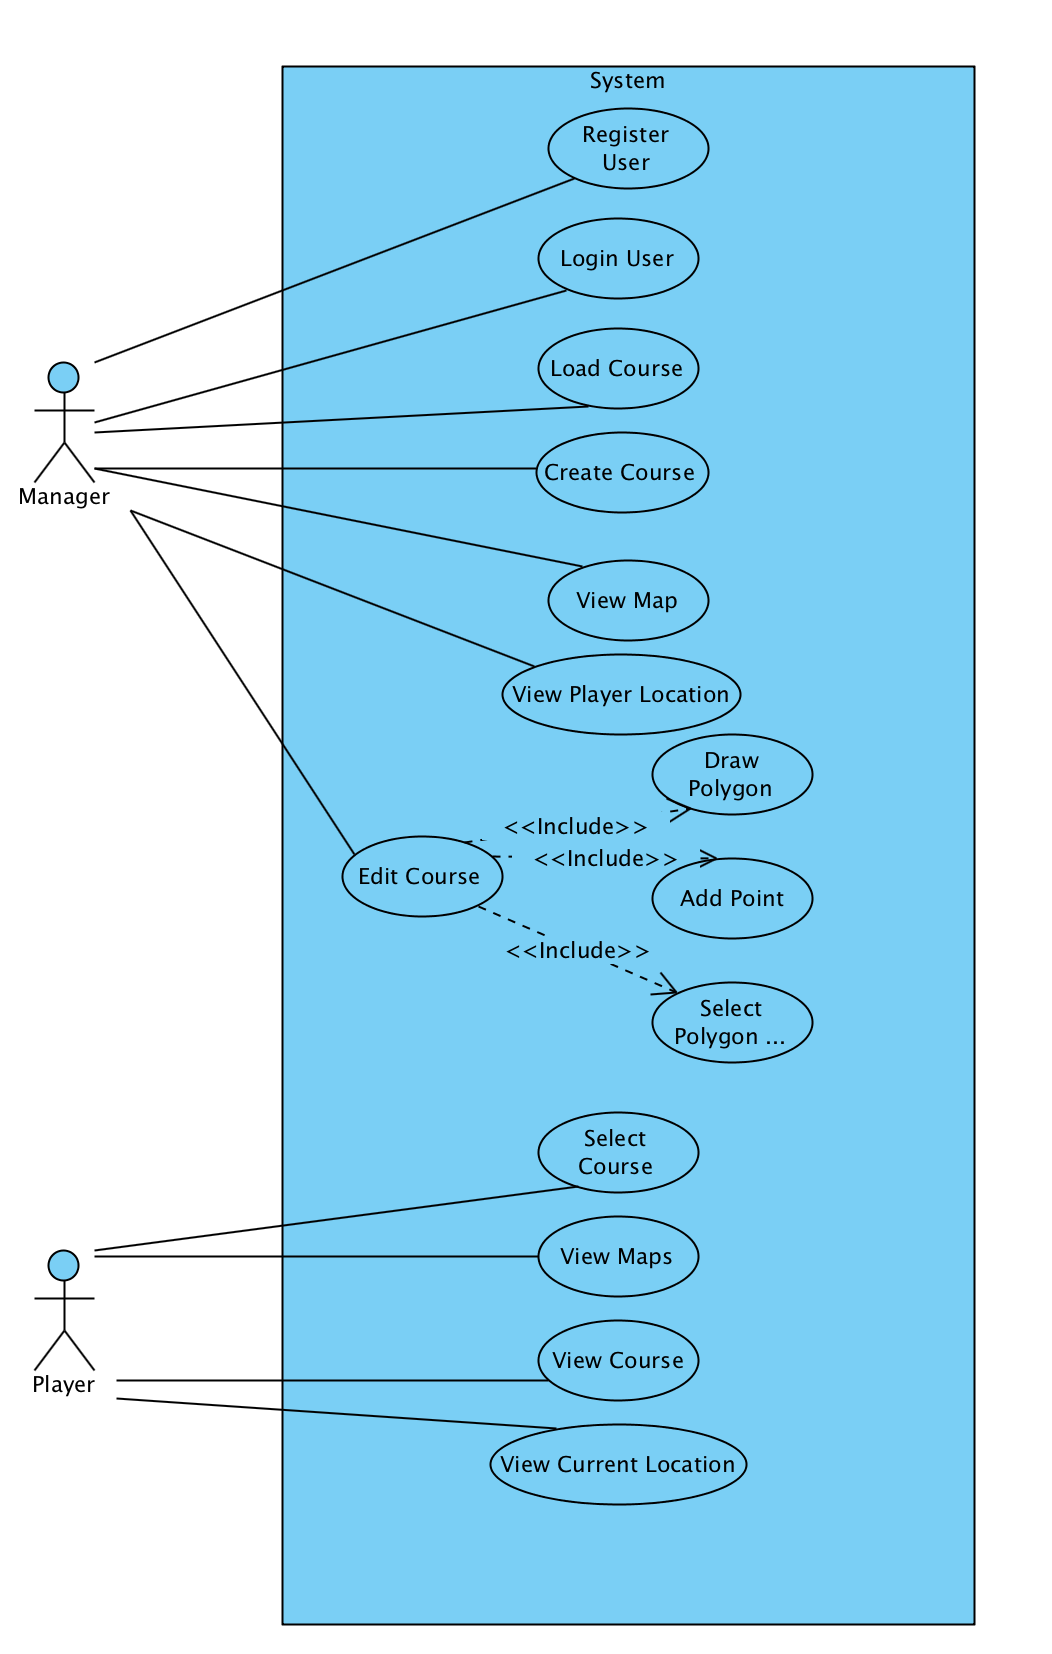
\includegraphics[scale=0.6]{UsecaseDiagram}
        \caption{Use case diagram illustrating user stories.}
        \label{fig:usecase}
    \end{figure}

    \newpage

    %===========================================================================

    \section{Non-Functional Requirements}

    The following sections each describe different non-functional requirements
    and briefly explain how these requirements are tested.

    \subsection{Performance Requirements}

    The system must be optimized to make as few Google Maps API calls as
    possible. The Google Maps API allows 25000 calls per day, after which the
    calls are billed.

    The performance is tested using stress testing, as layed out in the
    \textit{Testing Policy} [1].

    \subsection{Usability Requirements}

    Both the mobile applications and the web application must be made as user
    friendly as possible in order to appeal to a large audience. The users of
    the system will mostly have little to no technical background and must
    therefore be intuitive to use.

    A tutorial video must also be provided to ensure that users can have a brief
    introduction to the system.

    Usability is tested through usability tests, as explained in the
    \textit{Testing Policy} [1]. Briefly, this is done by presenting the web
    application or mobile application to different users, having them use the
    system and providing feedback at the end of the session.

    \subsection{Security Requirements}

    The API must be secure and must not allow unauthorized users to modify or
    remove courses, holes or elements. Furthermore, the API must not allow
    authorized users to modify courses, holes or elements belonging to a
    different user. Any user must be able to get read access to the courses,
    holes and elements and need not be authorized in order to do this. This is
    because the mobile applications' users are kept anonymous and do not
    require any identification or authorization.

    Security is tested through\ldots

    \newpage

    %===========================================================================

    \section{Architecture}

    \subsection{Interfaces}

    The next sections each describe the interfaces present in each specific
    subsystem.

    \subsubsection{Android Application}

    \begin{itemize}
        \item \textit{User:} The Android application interfaces with the user
            through the mobile device's screen. The user's input is used to
            navigate the map and choose holes to view. The user is also
            presented with a map displaying the course and additional info.
        \item \textit{Network:} The application interfaces with the networking
            devices of the mobile device. Network connection is required to use
            both the Zoning and Google Maps APIs.
        \item \textit{Zoning API:} The Zoning API is used to receive
            information on mapped courses, which is then displayed to the user.
        \item \textit{Google Maps API:} In order to display the information
            obtained from the Zoning API, the Google Maps API is used. The API
            allows the map to be displayed and displays the polygons and points
            on the map. The user's location is also obtained through the same
            API.
    \end{itemize}

    \subsubsection{iOS Application}

    \begin{itemize}
        \item \textit{User:} The iOS application interfaces with the user
            through the Apple device's screen. The user's input is used to
            navigate the map and choose holes to view. The user is also
            presented with a map displaying the course and additional info.
        \item \textit{Network:} The application interfaces with the networking
            devices of the Apple device. Network connection is required to use
            both the Zoning and Google Maps APIs.
        \item \textit{Zoning API:} The Zoning API is used to receive
            information on mapped courses, which is then displayed to the user.
        \item \textit{Google Maps API:} In order to display the information
            obtained from the Zoning API, the Google Maps API is used. The API
            allows the map to be displayed and displays the polygons and points
            on the map. The user's location is also obtained through the same
            API.
    \end{itemize}

    \subsubsection{Web Application}

    \begin{itemize}
        \item \textit{User:} The web application interfaces with the user
            through the browser's display. The user is presented with various
            controls and UI elements that are used to edit courses. The user is
            also presented with a satellite map for displaying and drawing
            courses, as well as active player's locations.
        \item \textit{Zoning API:} The Zoning API is used to receive
            information on mapped courses, which is then displayed to the user.
            The Zoning API is also used to create, modify or delete existing
            courses, holes or map elements.
        \item \textit{Google Maps API:} In order to display the information
            obtained from the Zoning API, the Google Maps API is used. The API
            allows the satellite map to be displayed and displays the polygons
            and points on the map. The API is also used to draw the elements on
            the map. 
    \end{itemize}

    \subsubsection{Zoning API}

    \begin{itemize}
        \item \textit{API/DBMS:} The API and the DBMS interface with one
            another through the server's internal network. The API connects to
            the DBMS in order to execute queries to create, receive, update or
            delete data.
        \item \textit{Network:} The API interfaces with the networking devices
            of the server. Network connection is required in order to
            communicate with the views, as explained in Section
            \ref{sec:sysarch}.
    \end{itemize}

    \subsection{Styles}

    \subsubsection{System Architecture}
    \label{sec:sysarch}
    
    The system is designed according to the MVC (Model-View-Controller)
    architectural pattern. This pattern is a good choice for the system as
    there is a single database responsible for storing information regarding
    mapped courses and there are multiple views that users interface with.
    
    The MVC pattern allows the abstraction of the model from the views, and
    also protects access to the model by the use of a controller. The
    abstraction created by the controller also increases the ease of
    maintaining the connection between the views and the model.

    Figure \ref{fig:depdia} shows the deployment diagram of the system and its
    subsystems. The different components of the MVC pattern are then following:

    \begin{itemize}
        \item \textbf{Model} - The DBMS serves as the model component by
            persisting the information required by the system. The DBMS is
            solely and exclusively responsible for the storage and retrieval of
            data, as well as enforcing integrity rules on the dataset.
            Information to be persisted includes the zones, areas, points and
            live location history of players.
        \item \textbf{Views} - The Android app, iOS app and website all serve
            as different views. The website is a view that uses the controller
            to read, create, update and destroy data stored within the model in
            order to manage the mapping of courses. The Android and iOS apps
            are simpler views with the sole purpose of fetching and displaying
            data received from the model via the controller, and calculating
            contextual information based on the received data.
        \item \textbf{Controller} - The API serves as the controller. It acts
            as a level of abstraction between the model and the views by
            controlling the access to the model. For a complete listing of the
            API endpoints, see the \textit{Swagger Documentation} [2].
    \end{itemize}

    \subsubsection{Zoning API Architecture}

    The Zoning API is designed as a persistence framework architecture. This
    architecture is a good choice for the API as it allows the hiding of the
    specific database implementation from the business objects.

    This also allows the separation of the database access from the actual
    implementation of the database, which enables easy maintenance, replacement
    and even distribution of the database. The different compoments of the
    persistence framework are listed as the following:

    \begin{itemize}
        \item \textbf{Database} - The DBMS serves as the database which can
            store business objects (in this case, courses and their elements).
            The database is solely responsible for persisting objects.
        \item \textbf{Database Manager} - The API serves as the database
            manager and controller, which abstracts the implementation of the
            database by providing a fixed set of functions that can be
            performed with persisted objects.
    \end{itemize}

    In order to allow the reuse of the Zoning API in generic mapping
    applications, the objects handled by the API are designed as a composite
    structure, as Figure \ref{fig:composite} shows. Every zone can have child
    zones and hold any amount of elements. This structure allows the API to be
    used for arbitrary zone mapping, with a specific application to the Golf
    Course Mapper system where a Hole is a child zone of a Course.

    \begin{center}
        \begin{figure}[H]
            \centering
            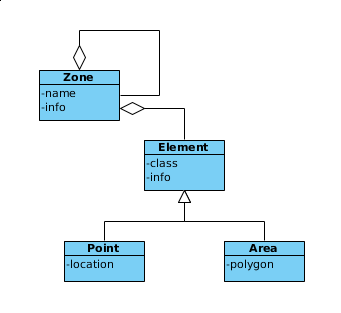
\includegraphics[scale=0.6]{Composite}
            \caption{UML Class Diagram illustrating the composite structure of
                the API objects.}
            \label{fig:composite}
        \end{figure}
    \end{center}

    \subsection{Configuration}

    The Web Application and Zoning API will both be hosted on a Amazon Web
    Services (AWS) Ubuntu Server. This includes the PostgreSQL DBMS, .NET Core
    Entity Framework and the Angular web service.

    The Android app will be available on the Google Play Store for download
    [3] on any mobile device that hosts an Android system with a minimum
    version of 4.4 (KitKat). The iOS app will not be available on the app
    store, but will be available on the GitHub repositories for installation on
    any Apple device. Finally, the web application will be available through a
    public URL [4] that can be accessed by any course manager that wishes to
    use the web application.

    The deployment diagram in figure \ref{fig:depdia} illustrates the
    configuration of the system.

    \begin{center}
        \begin{figure}[H]
            \centering
            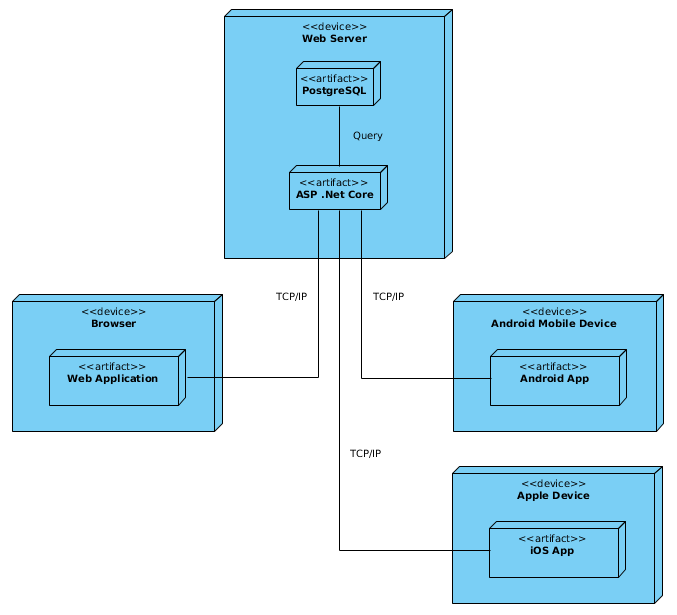
\includegraphics[scale=0.5]{DeploymentDiagram}
            \caption{Deployment diagram illustrating system configuration.}
            \label{fig:depdia}
        \end{figure}
    \end{center}

    \newpage

    \section{References}

    \begin{enumerate}
        \item Testing Policy
        (\url{https://github.com/team-recursive-recursion/documentation/raw/master/publish/testing-policy.pdf})
		\item Swagger Documentation
		(\url{http://ec2-18-191-152-232.us-east-2.compute.amazonaws.com/swagger}
		\item Android App Play Store
		(\url{https://play.google.com/store/apps/details?id=recrec.golfcourseviewer})
		\item Web Application
		(\url{http://ec2-18-191-152-232.us-east-2.compute.amazonaws.com})
    \end{enumerate}

\end{document}
